%!TEX root = ../masters_thesis.tex

% TODO: all examples as close as possible to the actual domain

\chapter{Basics} % (fold)
\label{cha:basics}

This chapter will lay the theoretical foundation of this Master's Thesis and will embed it into the context of current research. The title of this work is:

\vspace{-1em}
\begin{center}
\textbf{\titleFirst \\ \titleSecond}
\end{center}

It includes the domain (\emph{history of countries}) and the system to acquire, model, manage and visualize data of the domain: \emph{Historical Geographic Information Systems} (HGIS).

The first section of this chapter will define HGIS and related terms. Afterwards, concepts to model time and space in an information system are introduced. Data sources suitable for input into an HGIS are listed in the next section, followed by techniques to manage and analyse the data.
%A special focus lies on concepts to visualize spatial and temporal data, explained in the next section. The chapter closes with possible HGIS applications and introduces the tool that is used in this thesis: HistoGlobe.

extension of Hivent model to actors

% TODO: country definition
% TODO: enclaves and exclaves


% ==============================================================================
\section{Historical Geographic Information Systems} % (fold)
\label{sec:historical_geographic_information_systems}

\begin{quoteit}
  ``All human actions takes and makes place. The past is the set of places made by human action. History is a map of these places. The past thus exists not in time but in space.''
\end{quoteit}
\hfill -- Philip J. Ethington in \cite[précis]{citeTakeMakePlace}

An Historical Geographic Information System helps to answer research questions about how geographical phenomena have developed over time. To understand how it works, it is important to understand the four parts of the word: The research fields \emph{history} and \emph{geography} and the concepts of \emph{information} an \emph{systems}.


% ------------------------------------------------------------------------------
\subsection{History} % (fold)
\label{sub:history}

History is ``an ideal field for thinking long and hard about important questions''
\cite{ahaFiveCs}.
The Greek word \emph{\textIota\textsigma\texttau\textomikron\textrho\textiota\textalpha / historia}, meaning ``finding out, learning through research, narration of what is learned'', is the origin
\footnote{
  \emph{History},
  Dictionary.com, based on Random House Dictionary, 2015,
  URL: \url{http://dictionary.reference.com/browse/history},
  last access: 23.10.2015
}
and it signifies the two main modern usage forms of the term: To research about and learning something and to tell a story. There are many different definitions of the word \emph{history}
\footnote{
  \emph{History},
  Merriam Webster -- an Encyclopædia Britannica Company,
  URL: \url{http://www.merriam-webster.com/dictionary/history},
  last access: 23.10.2015
}.
The main goal of history is to study processes in the past to understand the situation in the present and make reasonable decisions for the future. The American Historical Association has developed the ``five C`s of historical thinking [that] together describe the shared foundations of [the] discipline''\cite{ahaFiveCs}:

\vspace{-1em}
\begin{description} % manipulation of indentation
  \item[Change over time]
  The lives of people, their languages and their cultures are continuously changing. Describing these historical changes, triggered by historical events happed in the past, is a major goal of history. Snapshots in the form of historical maps or historical photography are used to tackle this task.
  %TODO: refer to this in later sections
  \item[Context]
  is an important element of historical thinking. The goal is to travel back in time to the moment of the event and recreate the world based on primary sources. The understanding of the historical context is crucial for the understanding of the event.
  \item[Causality]
  The overall goal of each science is to answer the \emph{why}-question concerning an event or a process. For historians that means to reasonably explain an historical event or process based on evidence. The problem is that history is not a science that can alter experimental conditions to extract new information, in a way that e.g. experiments in physics work. Historians have to focus on the interpretation of primary sources, which inherently yields multiple explanations for a single event.
  \item[Contingency]
  is a derived aspect from this problem. Each event has a whole network of prior conditions, because the world is highly interconnected. A slight change in one prior condition could have led to a completely different outcome of the event and a different state of the world.
  \item[Complexity]
  The intrinsic human need for order conflicts with the complexity of history and their events and processes, because of its contingency. It is questionable if all details about events in the world are scientifically explainable.
  %This problem is comparable to the Heisenberg problem in physics: Whereas on the macro-level e.g. physical movements are a direct cause of a set of preconditions (speed, fraction, wind, weight, ...) and are therefore predictable, the smallest of all particles are not traceable, their movements are not predictable and therefore their processes not explainable.
\end{description}

Historical research is conducted by studying and interpreting primary sources, such as written documents, verbal texts, speeches, photographs, audio, video or historical maps. This signifies that most historical research is qualitative. The main organization principle in history is periodization: classifying events and processes to describe broader long-term changes and to explain complex phenomena
\cite[pp.4-7]{knowles2008placing}.
A special focus in this thesis is laid on historical maps as primary source to extract spatial information.

% subsection history (end)

% ------------------------------------------------------------------------------
\subsection{Geography} % (fold)
\label{sub:geography}


The term ``geography'' comes from Greek ~\emph{\textgamma\textepsilon\textomega\textgamma\textrho\textalpha\textphi\textiota\textalpha / geographia}~, literally ``describing the earth.''
\footnote{
  \emph{Geography},
  Dictionary.com, based on Random House Dictionary, 2015,
  URL: \url{http://dictionary.reference.com/browse/geography},
  last access: 23.10.2015
}
It is a science that studies the interplay between the landscapes and environments of the Earth (\emph{physical geography}) on the one hand and the people, their cultures, societies and economies (\emph{human geography}) on the other. That means geography is an interdisciplinary field between natural and social sciences
\cite{rgsGeography}.

Geographical research aims to understand where things are found, why they are there and how they developed over time.
% In regional geography, another subbranch, also the causes of social or environmental differences between cultures and landscapes want to be found.
It focuses on the interconnectivity between elements of physical and human geography, which gets expressed in Tobler's First Law of Geography: ``Everything is related to everything else, but near things are more related than distant things.''
\footnote{
  ``A computer movie simulating urban growth in the Detroit region'',
  Waldo Tobler, 1970
  Economic Geography, 46(2): 234-240.
}

Geographers use different technology and techniques to analyze geographic processes and to answer their research questions. The oldest and most important among those are maps. A map is a graphical expression of something that is not tangible: a part of the real world. A map shows the physical, environmental, political, economical or social properties of the Earth in order for the user of the map to get the most relevant information for his task, may it be orientation, learning or teaching. The ``art and science of making maps'' is the field of \emph{cartography}
\footnote{
  \emph{History of maps and cartography},
  James S. Aber,
  URL: \url{http://academic.emporia.edu/aberjame/map/h_map/h_map.htm},
  last access: 24.10.2015
}. Since maps visualize a model, they have a natural constraint: ``No map can perfectly replicate the real world, since it inevitably generalizes, abstracts and approximates the complexity of the reality''
\cite[p. 181]{knowles2008placing}.

% TODO:                 had? had? has had? is having?
% The scientific background of GIS is \emph{geographic information science} (GISci) that studies patterns in natural and human development, e.g. erosion of valleys, literacy rate, natural hazards and deals with approaches and techniques to manage, analyze and visualize this information
% \cite{ngGeography}.


\paragraph{Comparison between geography and history} % (fold)
\label{par:comparison_of_geography_and_history}

Both research fields utilize maps for answering their research questions, which is the main commonality for the work of this thesis. However, the nature of both fields are also very different, illustrated in table \ref{tab:history_vs_geography}.

\begin{table}[ht]
\begin{center}
\begin{tabular}{p{0px} r c l p{0px}}
    \toprule
    & geography
    & difference
    & history
    & \\
    \midrule
    & where
    & dimension
    & when
    & \\

    & exact, statistical
    & character
    & complex, fuzzy
    & \\

    & mainly quantitative
    & research
    & qualitative
    & \\

    & spatial proximity of conditions
    & causal explanation
    & temporal sequence of events
    & \\

    & spatial differentiation
    & explanation
    & temporal differentiation
    & \\

    & clustering
    & ordering
    & periodization
    & \\

    & mostly visual (maps)
    & expression
    & mostly verbal (texts)
    & \\

    & high (GIS)
    & digitalization potential
    & low (digital humanities)
    & \\
    \bottomrule
\end{tabular}
\caption{differences between history and geography \cite[pp. 2-4]{knowles2008placing}}
\label{tab:history_vs_geography}
\end{center}
\end{table}


Whereas geography answers the questions \emph{where?}, history focuses on \emph{when?} -- but the ultimate goal for both sciences is to answer the question \emph{why?}

% paragraph comparison_of_geography_and_history (end)


% subsection geography (end)

% ------------------------------------------------------------------------------
\subsection{Information} % (fold)
\label{sub:information}

The terms ``signs'', ``data'', ``information'' and ``knowledge'' are sometimes used interchangeably and there is no coherent definition for any of them. However, all describe different concepts. This explanation seen in figure \ref{fig:information} is based on the work of \cite{datinfwis}.

\begin{figure}[ht]
  \vspace{1em}
  \begin{center}
    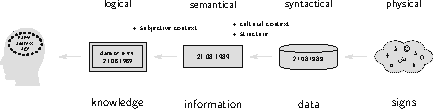
\includegraphics[width=0.9\textwidth]{graphics/basics/information}
  \end{center}
  \caption{signs, data, information and knowledge}
  \label{fig:information}
\end{figure}

A \emph{sign} is the physical representation of something in the real world. Since the real world is continuous, literally anything can be seen as a sign, so there are uncountably infinitely many different signs. \emph{Data} is a subset of all possible signs and represents the syntactical level of what an information system deals with. Data itself does not have any meaning, but as soon as it is organized, it becomes \emph{information}. However, information is sensitive to its cultural context. The string ~\texttt{14.07.1789}~ is useful and understandable for people in countries that use the date format \texttt{DD.MM.YYYY}. However, for people in Belize and the USA, that use the format \texttt{MM.DD.YYY}, this might just be a random string of numbers without any meaning, and therefore no information -- although it is the same data. If information is visualized to and understood by a human and it can be integrated into his or her larger subjective context, it is \emph{knowledge} \cite{nake}. The goal of a visualization is to present as much information as possible in a way that it can be transformed into knowledge by the viewer.

% subsection information (end)

% ------------------------------------------------------------------------------
\subsection{System} % (fold)
\label{sub:system}

A \emph{system} is an organized structure containing \emph{elements} or \emph{components} that are directly or indirectly \emph{related} to and \emph{interconnected} with each other. The elements and their relations form the whole of the structure. The surrounding of the system is its \emph{environment}. There is an \emph{internal state} at any point of the system's existence. This state only changes when it gets influenced by stimuli of its environment. \emph{Emergent properties} characterize a system. They are independent from properties of the element of the system, e.g. water is liquid at room temperature, but the elements it consists of, hydrogen and oxygen, are a gas. Each system is both part of a larger system and can be decomposed into subsystems. Therefore, systems form a hierarchy.

A system has defined spatial and temporal boundaries. There are two types: \emph{open systems} allow exchange of energy or information with their environment, whereas idealized \emph{close systems} naturally do not interact with and are not influenced by its environment. Based on the black box principle the inner working of a closed system can not be seen from the outside
\cite{system}.

% subsection system (end)

% ------------------------------------------------------------------------------
\subsection{Motivation} % (fold)
\label{sub:motivation}

An \emph{information system} (IS) is an application that is dealing with the acquisition, management, analysis and presentation of information. It is the unity of all its components and their interaction with each other
\cite{informationSystem}.
If the majority of the information in a system has a spatial relation to the Earth, its surface, its lithosphere, atmosphere or the social or economical structure of its habitation, it is a \emph{geographic information system} (GIS). The data objects in the system are called \emph{geo-objects}
\cite{bolstad2008gis}.
If the information additionally has a temporal dimension, e.g. via time stamps or time spans, which enable to trace developments of geo-objects, it becomes an \emph{Historical Geographic Information System}
\cite{gregory2014toward}
or alternatively \emph{Spatio-Temporal Information Systems} (STIS)
\cite{pelekis04stdms}.

HGIS react on the spatial turn of history: the integration of geographic methods in historical research. It aims to discover the power of cartographic representation: ``The spatial turn in the humanities must [...] understand the role of space in human events''
\cite{bodenhamer2010spatial}.
At the same time, they are the product of the temporal run in GIS: the coexistence of space (where things are) and time (what has changed over time)
\cite[p. 45]{solana2014spatio}.
With HGIS it is possible to analyze how ``spatial patterns change over time in order to better understand large-scale Earth processes''
\cite{peuquet99}.
Since ``the world never stands still'', but ``the retention of information relating to past events [is] an important element of human representation of the world'', the dimension of time has to be integrated into a GIS
\cite{peuquet99}.

HGIS are rather recent tools and used mostly in \emph{Digital Humanities} as a digital tool to answer research questions in the traditional fields of humanities: ``situating history in its geographical context and using geographic information to illuminate the past''
\cite[p. 3]{knowles2008placing}.
Some interesting research questions that could be answered using HGIS could be:

\begin{compactitem}
  \item Did the European Union help to bring peace on the European continent?
  \hfill \emph{(political)}
  \item Is there a coherence between life expectancy and fertility rate?
  \hfill \emph{(social)}
  \item What is the effect of global warming on the melting of glaciers?
  \hfill \emph{(physical)}
  \item What was the effect of Bismarck's foreign policy on peace in Europe?
  \hfill \emph{(historical)}
\end{compactitem}

Or on a more abstract level: Where and When has something changed and why did it change?

% subsection motivation (end)

% ------------------------------------------------------------------------------
\subsection{Components} % (fold)
\label{sub:components}

Information systems in general are based on a data model --- HGIS in particular on a \emph{spatio-temporal data model}, introduced in section \ref{sec:spatio_temporal_data_models}. On top of that, there are different components. One way to classify them is using the four-component model:

\begin{enumerate}
  \item \textbf{Input}: Primary acquision of spatio-temporal data, i.e. historical events, historical and current countries and their territories.
  \item \textbf{Management}: Physical storage and logical management of the data in a spatio-temporal database, using a structure that fits the spatio-temporal data model.
  \item \textbf{Analysis}: Gaining spatio-temporal information by cleaning, transforming or combining the data in database.
  \item \textbf{Presentation}: Visualization of information on different displays, e.g. a map and a timeline, transforming information into spatio-temporal knowledge.
\end{enumerate}

% subsection components (end)

% ------------------------------------------------------------------------------
\subsection{Applications} % (fold)
\label{sub:applications}

``Today, operational temporal GIS does not exist''. This quote summarizes the state of the art in this field. The main reasons are ``the complexity of integrating space and time and the lack of standards''
\cite[p. 5]{raza12}.

However, there are numerous project that use HGIS for one specific research question. A large collection them can be found in \cite{knowles2008placing} and \cite{gregory2014toward}. A famous visualization combining time and space Napoleons Moscow Campaign by Charles Minard from 1869 (see figure \ref{fig:minard_napoleon}). The ``best statistical graphic ever drawn''
\footnote{
  \emph{The Visual Display of Quantitative Information} (p. 40),
  Edward R. Tufte,
  2001
}
shows the number of men in Napoleon’s 1812 Russian campaign army, their movements, as well as the temperature they encountered on the return path
\cite[pp. 188-191]{knowles2008placing}.

\begin{figure}[ht]
  \centering
  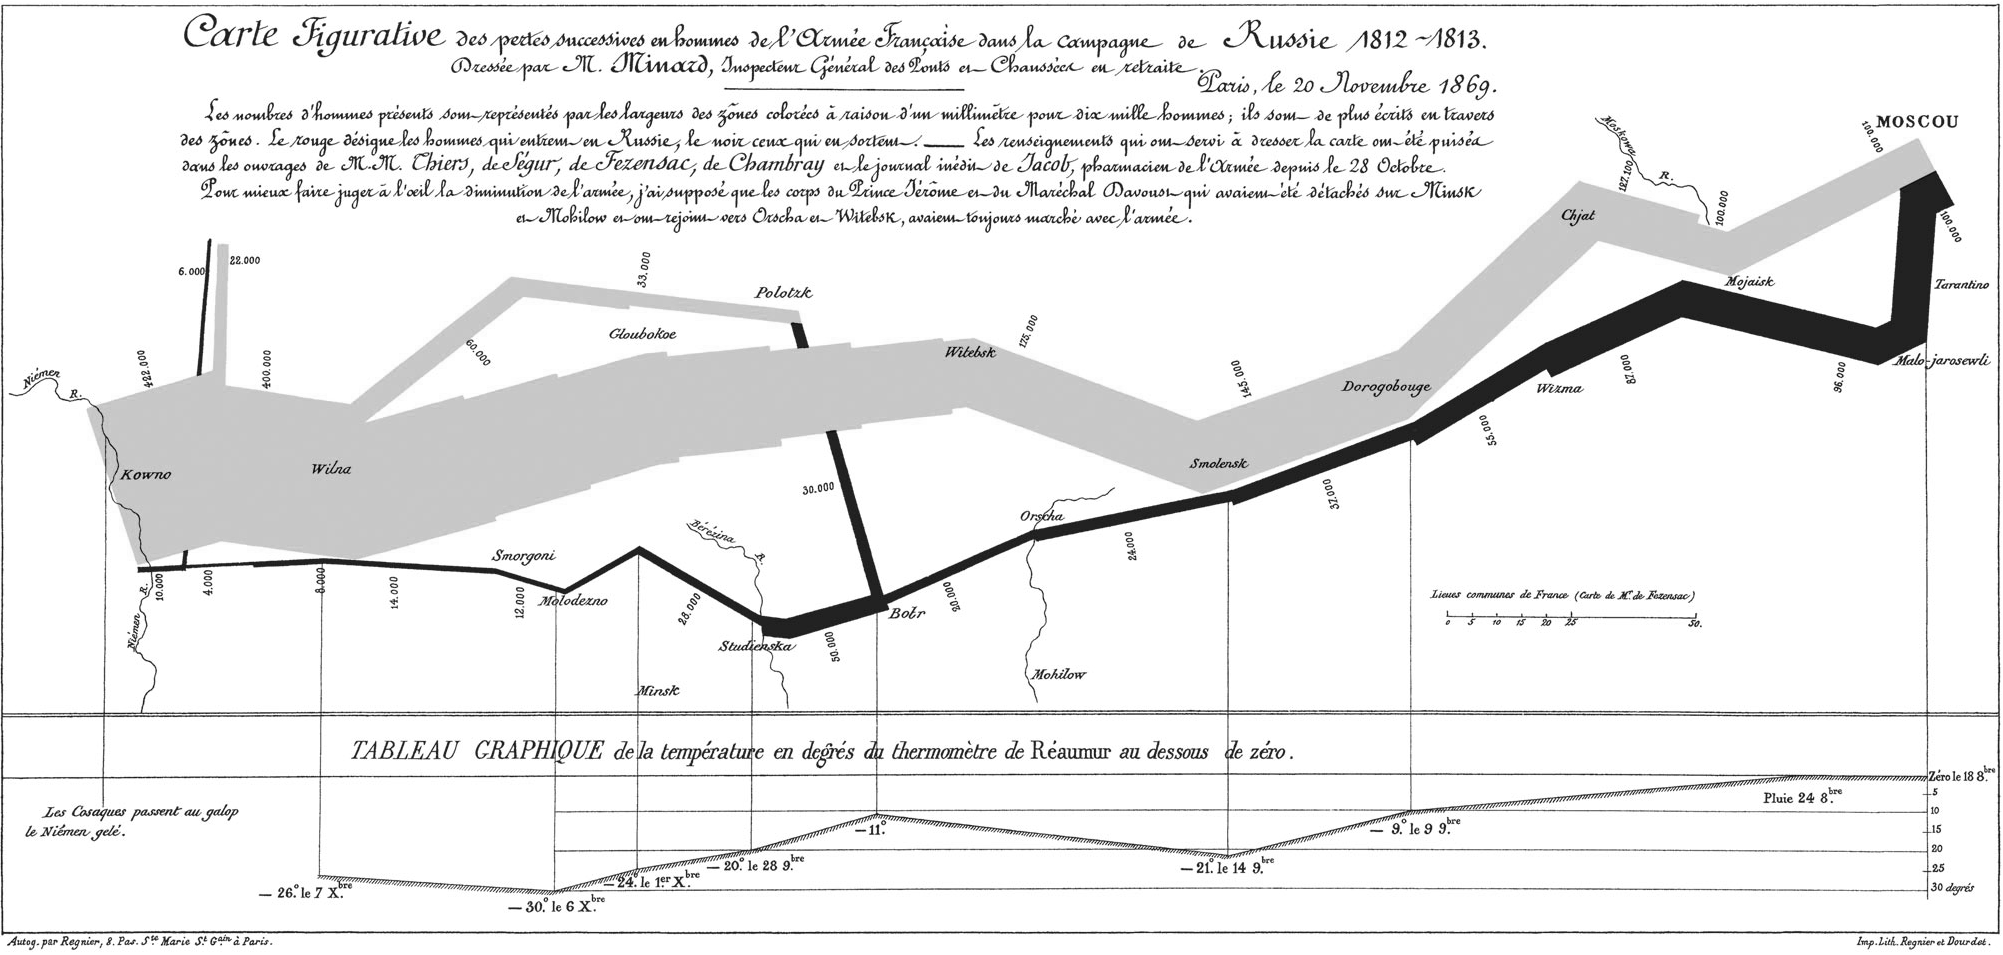
\includegraphics[width=0.8\textwidth]{graphics/basics/napoleon_march_moscow.png}
  \caption{Napoleons Moscow Campaign \protect\footnotemark}
  \label{fig:minard_napoleon}
\end{figure}

\footnotetext{
  \emph{Minard.png}
  Charles Minard, 1869,
  URL: \url{https://commons.wikimedia.org/wiki/File:Minard.png},
  last access: 03.11.2015,
}

The \emph{Great Britain Historical GIS Project} (GBHGIS)
\footnote{
  \textit{Great Britain Historical Geographical Information System (GBHGIS)},
  Ian Gregory \& Humphrey R. Southall, University of Portsmouth, since 1994,
  URL: \url{http://www.port.ac.uk/research/gbhgis/},
  last access: 02.11.2015
}
combines statistical data with territorial units of the United Kingdom, e.g. to analyze net migration in the districts in UK. The data is collected by the \emph{British Ordnance Survey}, who automatically detect spatial changes to the geography and land use of the United Kingdom using aerial photography
\footnote{
  \textit{British Ordnance Survey},
  URL: \url{https://www.ordnancesurvey.co.uk/education-research/research/automatic-change-detection.html},
  last access: 02.11.2015
}.

The \emph{National Historical Geographic Information System} (NHGIS)
\footnote{
  \textit{Welcome to NHGIS},
  Minnesota Population Center, University of Minnesota,
  since 2007,
  URL: \url{},
  last access: 02.11.2015
}
provides the digital boundaries of the United States of America and census data for each year since 1790.
% \cite{aerialInterpolation}
While the data in the system is extensive, the interface to analyze and use the data is very frustrating to use: A tutorial is necessary to go through the selection process. To download data, a user has to register, receive an email with a link to download a compressed file which has to be decompressed and then loaded into a GIS software to be visualized.

HGIS are not widely accepted in the humanities. One reason is the nature of the qualitative historical research: historic sources are subjective and biased, their content may be fuzzy and they are definitely incomplete. So the knowledge that can be extracted from a source bears the integral problem of \emph{uncertainty}. Information systems on the other hand have a logical architecture and, to be as precise and accurate as possible. Analysis is based on mathematical functions -- an information system is quantitative in its entire nature
\cite[p. 2]{knowles2008placing}.

% subsection applications (end)

% ------------------------------------------------------------------------------
\subsection{Data Sources} % (fold)
\label{sub:data_sources}

This HGIS needs data about historical countries, their names and borders and historical events that lead to historical changes of these countries. There are a lot of free and open sources for geographic data about the current countries, their names and borders. One of the most exhaustive collections of geographic data in public domain is hosted by Natural Earth
\footnote{
  \textit{Natural Earth},
  URL: \url{http://www.naturalearthdata.com/downloads/},
  last access: 30.10.2015
}.
There is physical data (e.g. coastlines, rivers, or glacier areas) and cultural data (e.g. political borders, cities, roads, airports or timezones). OpenStreetMap also opens its database to the public
\footnote{
  \textit{Planet OSM},
  URL: \url{http://planet.openstreetmap.org/},
  last access: 30.10.2015
}.

However, data about historical countries and events are not as straightforward to aquire, because of the mostly qualitative nature of historical research (see section \ref{sub:history}). The most exhaustive free and open source of historical is the \emph{Wikipedia} and their article categories, e.g. \texttt{armistices} or \texttt{treaties}
\footnote{
  \textit{Category:Treaties},
  Wikipedia, the free encyclopedia,\\
  URL: \url{https://en.wikipedia.org/wiki/Category:Treaties},
  last access: 13.05.2016
}.
All sorts of historical events can be found, even translated into different languages. Some information is structured in information boxes, e.g. some historical treaties have a name, an image, a location, a signature and an effect date, an overview about treaty conditions and signatories. Particularily interesting for this thesis are articles about historical countries
\footnote{
  \textit{List of former sovereign states},
  Wikipedia, the free encyclopedia,
  URL: \url{https://en.wikipedia.org/wiki/List_of_former_sovereign_states},
  last access: 13.05.2016
},
because they contain the name of the country and meta information, e.g. their historical successors and predecessors. Building an open-source Historical Geographic Information System on the basis of Wikipedia would be a huge project with significant impact on the world of free and open education --- however, it would also be a big challenge: Wikipedia is incomplete, not all historical countries and events necessary to model the history of the world are available. It is also inconsistent, because not all articles about historical countries and events are structured, especially not to those who actually have an influence on a territorial change of a country, e.g. a border agreement. Retrieving, parsing and processing this information is a big challenge. Also the problem of accuracy and quality of information in the Wikipedia due to their open source nature has to be considered. Overall, using the Wikipedia as a data source for this thesis is not feasible, but is subject to further research.

% - - - - - - - - - - - - - - - - - - - - - - - - - - - - - - - - - - - - - - -
\paragraph{Historical maps} % (fold)
\label{par:historical_map}

The most problematic data to acquire is about the territories and borders of historical countries. There is no primary data source for that, so the only way to retrieve a border is to extract it from an historical map.

They also can be found on Wikipedia, or in historical map colletions, e.g. \emph{OldMapsOnline}. The project is developed ``out of a love of history and heritage of old maps'' and currently stores about 400000 historical maps
\footnote{
  \textit{Old Maps Online},
  URL: \url{http://www.oldmapsonline.org/},
  last access: 13.05.2016
}.
There are five steps to retrieve a border with points in geographic coordinates from an historical map.
\begin{enumerate}
  \item \textbf{Digitization}: If the map is on paper, it has to be scanned in the best possible quality. The result is a raster graphic.
  \item \textbf{Georeferencing}: The historical map has to fit as good possible on the reference map. This requires to manually define a set of reference points which are used to transform the map into the geographic coordinate system. This process is error-prone, especially if the projection of the historical map is not known and the map itself is not accurate
  \cite[pp. xvii]{knowles2002past}.
  The outcome is a raster graphic in which each pixel is assigned a geographic coordinate.
  \item \textbf{Preprocessing}: The raster image has to be be processed so that the desired border stands out and can be traced in the next step. This happens via greyscale conversion, thresholding or the Canny Edge Detector. This results in a monochrome graphic in which the desired border must be uninterrupted and clearly be seen.
  \item \textbf{Line detection}: By selecting a start and an end point of the border, the line gets traced automatically. This step vectorizes one particular feature, a borderline, from the raster graphic and produces a polyline in geographic coordinates.
  \item \textbf{Postprocessing}: In the last step, the polyline can be adapted: The line can be simplified to reduce unnatural artifacts and the position of border points can be manually edited. The final output of the whole process is a polyline whose points are expressed in the geographic coordinate system which can be used in the system as a border of an historic country.
\end{enumerate}

This process was developed in a preceding \emph{HiBo} project
\footnotetext{
  \textit{HiBo - semi-automatic extraction of borders from historical maps},
  Project of: B. Weber, N. K. Dankwa, K. Singh and T. Kashyappan, supervised by: Prof. Volker Rodehorst and Marcus Kossatz, Bauhaus-Universität Weimar, February 2015,
  URL: \url{https://bitbucket.org/bastian_weber/hibo},
  last access: 29.10.2015
}
(see figure \ref{fig:hibo}).

\begin{figure}[ht]
  \centering
  \begin{subfigure}{0.48\textwidth}
    \centering
    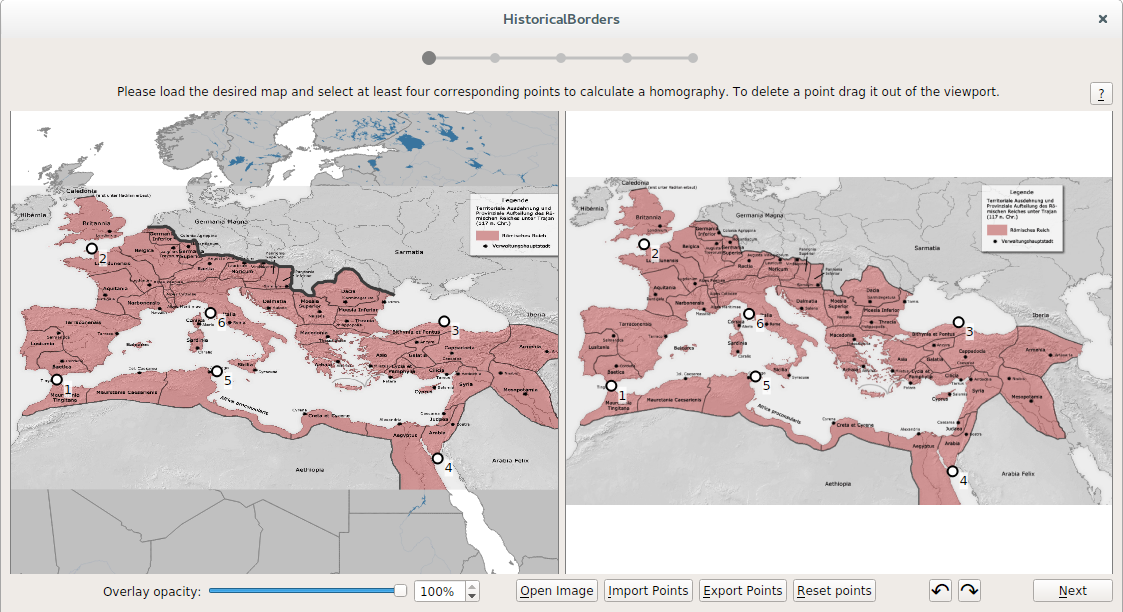
\includegraphics[width=0.95\linewidth]{graphics/basics/hibo1.png}
    \caption{Georeferencing}
  \end{subfigure}
  \begin{subfigure}{0.48\textwidth}
    \centering
    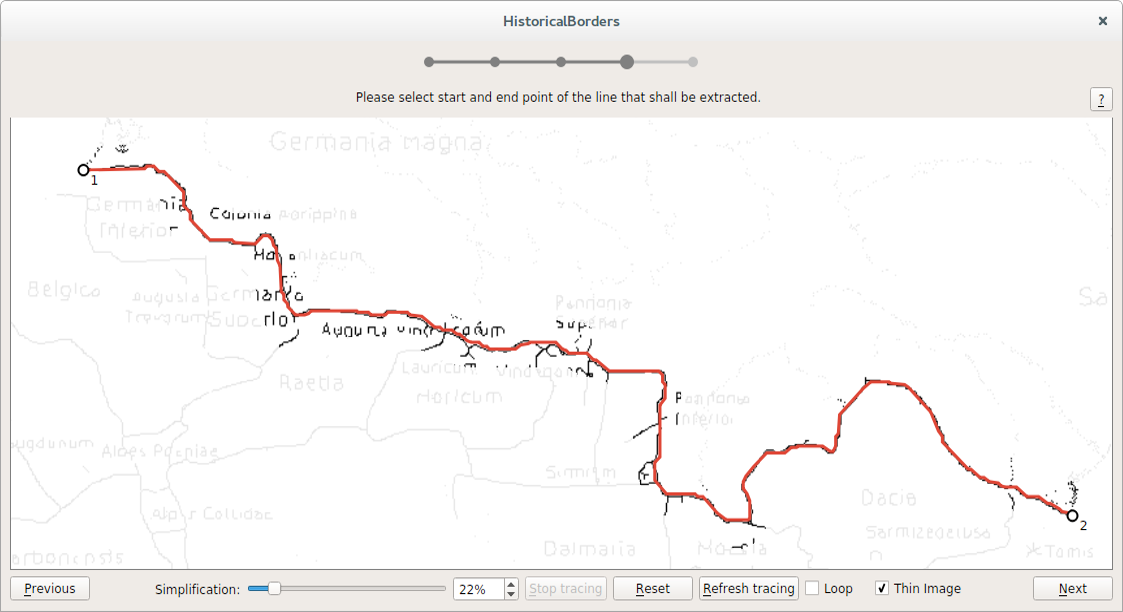
\includegraphics[width=0.95\linewidth]{graphics/basics/hibo2.png}
    \caption{Semi-automatic digitizing}
  \end{subfigure}
  \caption{Semi-automatic extraction of a border from a map of the Roman Empire \protect\footnotemark}
  \label{fig:hibo}
\end{figure}

% paragraph historical_map (end)

% - - - - - - - - - - - - - - - - - - - - - - - - - - - - - - - - - - - - - - -
\paragraph{Manual data input} % (fold)
\label{par:manual_data_input}

For the domain of this HGIS, the evolution of countries over time, there is no complete dataset available. Therefore, the system developed in this thesis needs to have an interface to enter historical data. The user needs to have an interface to enter information about historical events that change territories and names of historical countries. This data has to be acuired either from primary historical sources directly, or from free online sources. Next to Wikipedia, there are other collections of historical events, e.g. \emph{Correlates of War}
\footnote{
  \textit{Data Sets},
  Correlates of War,
  URL: \url{http://www.correlatesofwar.org/data-sets/folder_listing},
  last access: 13.05.2016
}
for quantitative data about international relations.


% paragraph manual_data_input (end)

% subsection data_sources (end)

% section historical_geographic_information_systems (end)

% ==============================================================================
\section{Time and Space} % (fold)
\label{sec:time_and_space}

This section will explain ways to separately represent time and space in an information system. It will first explain the geospatial data model used in traditional GIS and then introduce maps as the representation of spatial information. In the second part of the chapter, models to represent the temporal dimension are introduced.

% ------------------------------------------------------------------------------
\subsection{Model of Geographical Space} % (fold)
\label{sub:model_of_geographical_space}

HGIS need to unambiguously locate geo-objects on, underneath or close to the Earth's surface using \emph{geographic coordinates}. They express an object directly in the coordinate system of the Earth. To understand that, a model of the Earth has to be developed, the \emph{geodetic datum}, that needs to fit the real shape of the Earth as accurately as possible.

% - - - - - - - - - - - - - - - - - - - - - - - - - - - - - - - - - - - - - - -
\paragraph{The shape of the Earth} % (fold)
\label{par:the_shape_of_the_earth}

measured in the field of \emph{geodesy} is very complicated. In the Babylonian Empire ($\approx$ 2000-539 BC) the theory of the Earth being a flat disc surrounded by an infinite body of water
%(a theory still valid in some southern parts of the United States of America)
evolved. The Greek scientists Pythagoras and Aristotle (340 BC) rejected this theory and proved the earth to be a three-dimensional spherical object. It took almost 2000 years until Sir Isaac Newton (1687) reasoned that due to the centrifugal forces of the rotating Earth the shape has to be flattened at the poles and is therefore better described as an \emph{ellipsoid} with two radii: the polar radius ($r_p$) and the slightly larger equatorial radius ($r_e$)
\cite[pp. 69-77]{bolstad2008gis}.

However, the model disregards that the surface of the Earth is not flat but consists of deep oceanic trenches and high mountains. Therefore the gravitational field of the Earth is not homogeneous either: the actual \emph{mean sea level}, the reference surface for the height of objects varies from 106 meter below to 85 meter above the uniform sea level of the ellipsoid model. These discoveries in the \nth{20} century led to the complex \emph{geoid} model (see figure \ref{fig:geoid}). The latest and most accurate measurements for the shape of the Earth are the result of the GOCE satellite launched in March 2009
\cite{geoid, geoidESRI}.

\begin{figure}[H]
  \centering
  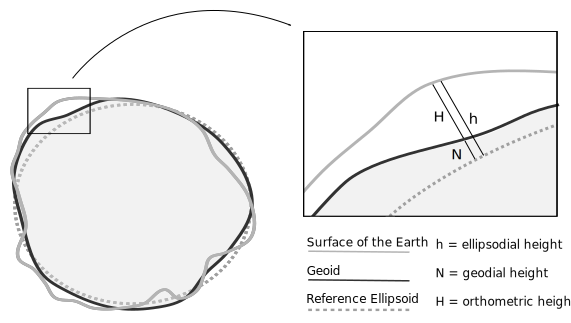
\includegraphics[width=0.72\textwidth]{graphics/basics/geoid}
  \caption{The geoid model, differences are exaggerated, \cite[Fig. 3-6, p. 75]{bolstad2008gis}}
  \label{fig:geoid}
\end{figure}

% paragraph the_shape_of_the_earth (end)

% - - - - - - - - - - - - - - - - - - - - - - - - - - - - - - - - - - - - - - -
\paragraph{Geographic coordinate system} % (fold)
\label{ssub:geographic_coordinate_system}

The basis for the geospatial data model is the reference ellipsoid. It is represented in a three-dimensional \emph{spherical coordinate system}. The \emph{North} and the \emph{South Pole} are defined as the two surface points closest to the Earth's center opposite to each other. The \emph{Equator} is the line equidistant to the two poles and dividing the world in a \emph{Northern} and \emph{Southern Hemisphere}. Additionally, the \emph{Prime Meridian} is defined as the line perpendicular to the Equator, running from the North to the South Pole. Since there are infinitely many lines like this, its definition is arbitrary, but by convention, the line running through Greenwich (London, United Kingdom) is used. Based on these two lines, each point in the spherical coordinate system can be unambiguously defined by
\cite[pp. 26-28]{bolstad2008gis}:

\begin{compactenum}
  \item The rotation angle along the Equator, defining its longitude: $\gamma = [-180\degree ~...~ +180\degree]$
  \item The rotation angle along the Prime Meridian, defining its latitude: $\phi = [-90\degree ~...~ +90\degree]$
  \item The distance to the origin: $r \in \mathbb{N}_0$
\end{compactenum}

\begin{figure}[ht]
  \vspace{1em}
  \centering
  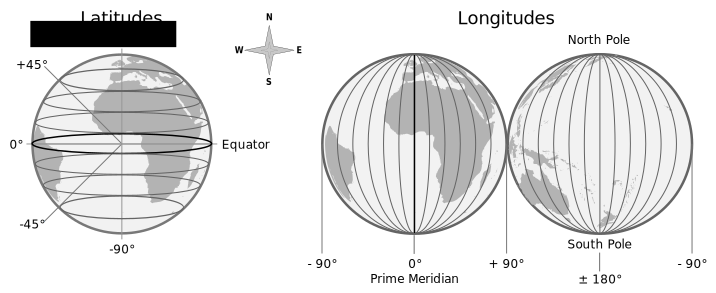
\includegraphics[width=0.8\textwidth]{graphics/basics/geo_coordinates}
  \caption{geographic coordinates using latitude and longitude}
  \label{fig:geo-coordinates}
\end{figure}

Lines of constant latitude are running horizontally and are called \emph{parallels}, lines of constant longitude are \emph{meridians} appearing in vertical direction. All parallels are circles with their center on the axis between the poles. No two parallels intersect. The longest parallel is the Equator (0\degree~latitude). All meridians have the same length. Geographic coordinates are usually recorded either in degree-minutes-second (\texttt{DMS}, e.g. \texttt{50\degree~58' 22''}) or in decimal degree (\texttt{DD}, e.g. \texttt{50.973}) notation
\cite[pp. 30, 79]{bolstad2008gis}.


% - - - - - - - - - - - - - - - - - - - - - - - - - - - - - - - - - - - - - - -
\paragraph{The Geodetic Datum} % (fold)
\label{par:geodetic_datum}

is the digital model of the analogue Earth. It consists of two parts: The approximation of the Earth's surface in a the Cartesian coordinate system with the origin in the Earth's center and a set of reference points used to accurately locate a point.

Geodetic datums can be very accurate in one region of the world, i.e. the model fits the real geoid very well, but inaccurate in another region. This is the main reason why there are a lot of different geodetic datums used in the world. The same coordinates in two different geodetic datums define two different points on Earth. In order to be accurate is essential to know the geodetic datum of the coordinates
\cite[p. 80]{bolstad2008gis}.
The \emph{World Geodetic System 1984 (WGS84)} is a model that found worldwide acceptance and is used in all major Web-based mapping services like \emph{OpenStreetMap} and in the GPS unit of major mobile devices.

% paragraph geodetic_datum (end)

% - - - - - - - - - - - - - - - - - - - - - - - - - - - - - - - - - - - - - - -
\paragraph{Raster and Vector Model} % (fold)
\label{ssub:raster_vs_vector_model}

The real world is infinite in detail, but storage in a computer system is finite. In order to model continuous geographical phenomena in an information system, a relevant subset of them has be sampled to create discrete spatial data. It can be represented in a raster or in a vector model.

\begin{figure}[H]
  \centering
  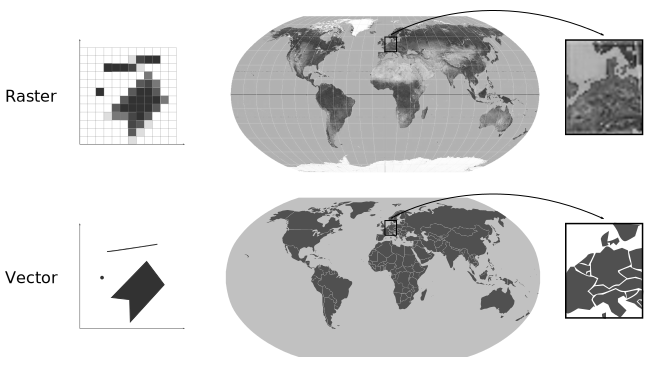
\includegraphics[width=0.75\textwidth]{graphics/basics/raster_vector}
  \caption{Comparison of the raster and the vector model}
  \label{fig:raster_vector}
\end{figure}

The \emph{raster model} contains a regular grid with a fixed \emph{cell dimension}. Each cell has a certain value, e.g. a color value.
The model is simple and allows straightforward rendering: only affine transformations have to be applied in order to project two raster map layers on top of each other. The main disadvantage of the raster model is its fixed resolution: it can not be scaled up without losing quality
\cite[pp.42-48]{bolstad2008gis}.
Raster graphics are used for map tiles by most map engines, e.g. in OpenStreetMap or the satellite image by NASA in Google Maps.
% \footnote{
%   \emph{Google Maps},
%   URL: \url{https://www.google.com/maps/@51.2090662,13.2328189,3563505m/data=!3m1!1e3},
%   Imagery \textcopyright2015 Landsat, Data SIO, NOAA, U.S. Navy, NGA, GEBCO, IBCAO, U.S. Geological Survey, Map data \textcopyright2015 Google, ORION-ME,
%   last access: 29.10.2015
% }.

In the two-dimensional \emph{vector model}, each object is a mathematically described geometric primitive. All of them can be expressed by three basic primitives (figure \ref{fig:geometric_primitives}):
\begin{enumerate}
  \item[0D] A \emph{point} is the fundamental object in vector geometry. It has no dimension, no size and is only defined by its position, specified in geographic coordinates. One point is independent from all others. Points can be used to represent the location of an event.
  \item[1D] A \emph{polyline} is constructed by an ordered set of points with at least one start and one end point. A border line can be expressed by a polyline.
  \item[2D] A \emph{polygon} is an ordered set of polylines creating a closed area. A polygon can be \emph{simple}, \emph{weakly simple} or \emph{complex} (see figure \ref{fig:polygon_properties}). The territory of a country without islands can be described by a polygon. If a country does have islands or overseas territories, a \emph{polypolygon} represents multiple separate polygons belonging to one logical entity.
\end{enumerate}

\begin{figure}[H]
  \centering
  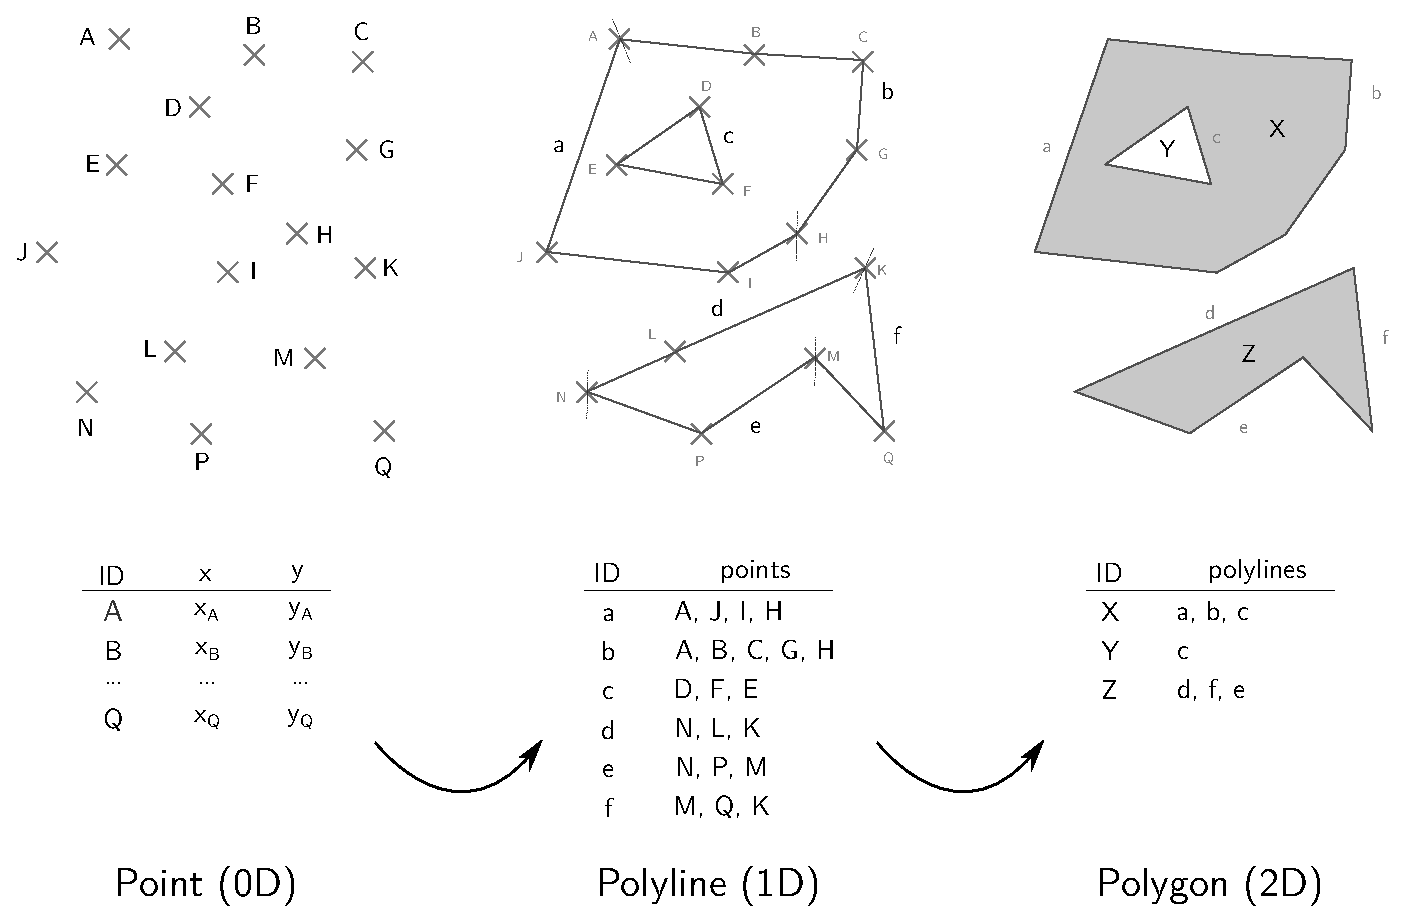
\includegraphics[width=0.8\textwidth]{graphics/basics/geometric_primitives}
  \caption{The basic geometric primitives point, polyline and polygon}
  \label{fig:geometric_primitives}
\end{figure}


\begin{figure}[H]
  \centering
  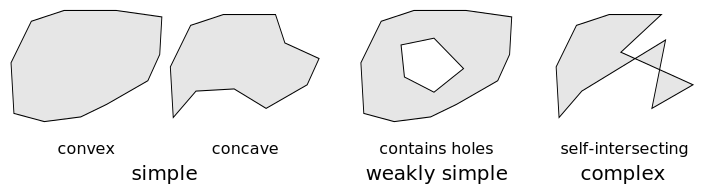
\includegraphics[width=0.5\textwidth]{graphics/basics/polygon_properties}
  \caption{Different properties of polygons}
  \label{fig:polygon_properties}
\end{figure}

Scale-independence is one of the biggest advantages of a vector model. The data model is more compact in comparison to the raster model. On the other hand, the model can become very complex. Since vector data has to be rasterized to be shown on the screen, the computational effort increases with complexity \cite[pp.33-42]{bolstad2008gis}.
Vector models are suitable to represent phenomena that can easily to discretized, e.g. the boundaries of a country. Common file types for vector data with spatial reference are the open file format GeoJSON (\texttt{.geojson})
\footnote{
  \emph{GeoJSON},
  IETF GeoJSON Working Group,
  URL: \url{http://geojson.org/},
  last access: 30.10.2015
}
% and Scalable Vector Graphics (\texttt{.svg})
% \footnote{
%   \emph{W3C SVG Working Group},
%   IETF Geographic JSON Working Group,
%   URL: \url{http://www.w3.org/Graphics/SVG/},
%   last access: 30.10.2015
% }
or ESRI Shapefiles (\texttt{.shp})
\footnote{
  \emph{ESRI Shapefile Technical Description},
  ESRI White Paper, July 1998,
  URL: \url{http://www.esri.com/library/whitepapers/pdfs/shapefile.pdf},
  last access: 30.10.2015
}.

% paragraph raster_vs_vector_model (end)

% - - - - - - - - - - - - - - - - - - - - - - - - - - - - - - - - - - - - - - -
% \paragraph{Geospatial Topology} % (fold)
% \label{par:geospatial_topology}

% \emph{Topology} is the study of position, how objects are spatially arranged and relatively positioned to each other. It does not include measures like distances or angles. Two objects are said to be topologically equivalent, if they can be deformed into each other, e.g. an ellipse can be stretched into a circle. A \emph{geospatial topological vector model} defines the relationship between geospatial objects, i.e. equals, disjoint, intersects, touches / neighbors, contains, covers, within, interior and boundary
% \cite{clementiniTopology}.

% The 2D vector model can be extended with a topology. The elements in this topological space are nodes (0D), edges (1D) and meshes (2D) and they correspond directly to the geometric primitives stated above. A topological vector model has strict connectivity (a ``clean'' geometry), if no two edges intersect without a node at their intersection point (planar), each interior edge has exactly two adjacent areas and each edge contains at least two nodes
% \cite[pp.37-39]{bolstad2008gis}.

% \begin{figure}[ht]
%   \centering
%   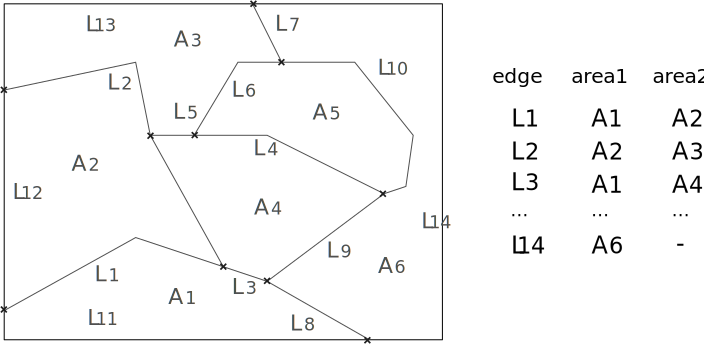
\includegraphics[width=0.55\textwidth]{graphics/basics/topological_vector_model}
%   \caption{An example of a topological vector model and an adjacancy table}
%   \label{fig:topological_vector_model}
% \end{figure}

% The topological vector model has a great asset: if an edge between two adjacent areas changes, the connectivity and adjacency does not change and therefore also the topology stays constant. The lookup for neighboring areas is very fast if the topology ensures strict connectivity: The neighbors of an area can be found in the adjacency table. Potentially problematic is the creation of a clean geometry: it can be cumbersome and require a lot of manual adjustment, for example ensuring strict connectivity by manually connecting nodes.

% % paragraph geospatial_topology (end)

% % subsection model_of_geographical_space (end)

% ------------------------------------------------------------------------------
\subsection{Presentation of Geographic Space} % (fold)
\label{sub:presentation_of_geographic_space}

The most common ways to present geographic space are two-dimensional \emph{maps} and three-dimensional \emph{globes}. The HGIS in this thesis will use a map to show the evolution of countries over time. A map is a discrete graphical expression of the geographical features of the continuous real world. The creation of a map is not just a scientific, but also a creative process: The form, function and interaction methods shall follow the purpose of the usage of the map.

A map is typically structured according to the \emph{layer} principle: Each layer is a transparent film showing one specific aspect, e.g. a physical layer showing coastlines, mountains or forests, a political layer showing international borders or a cultural layer showing cities or population densities. The layers are interchangeable, can be switched on and off and serve to serve a different visualization purpose. A \emph{legend} including the scale bar and north arrow shall explain all symbols used on the map and give orientation. In interactive web based systems, there should be \emph{menus} with different visualization options, e.g. panning and zooming on the map, switching map layers on and off or changing the color scheme of the map
\cite[pp. 159-166]{bolstad2008gis}.

\emph{Leaflet.js} is ``an open-source JavaScript library for mobile-friendly interactive maps''
\footnote{
  \textit{Leaflet - JavaScript library for interactive maps},
  URL: \url{http://leafletjs.com/},
  last access: 02.11.2015
}
that offers functionality to embed a map with a chosen projection in on the client-side of a web based information system, use own map tiles, symbols and markers on the map and tools for zooming and panning.

\paragraph{Map projections} % (fold)
\label{par:map_projections}

Since the Earth is three-dimensional, but the map on the computer screen only two-dimensional, the model of the Earth has to be projected onto the map. But as previously discussed in subsection \ref{par:the_shape_of_the_earth}, the Earth is an inhomogeneous spherical object with a curved surface whereas the map is flat
\cite[p.79]{bolstad2008gis}.
That is why some features of the Earth will be distorted on the map: An \emph{equivalent projection} preserves the area sizes of features on the map, whereas a \emph{conformal projection} preserves angles and the shapes of objects. Every map projection that is area-preserving distorts shapes at the same time, and each shape-preserving map distrots areas to some degree. There is no perfect map projection.
\cite{mapProjectionGeokov}.

\begin{figure}[ht]
  \centering
  \begin{subfigure}{0.59\textwidth}
    \centering
    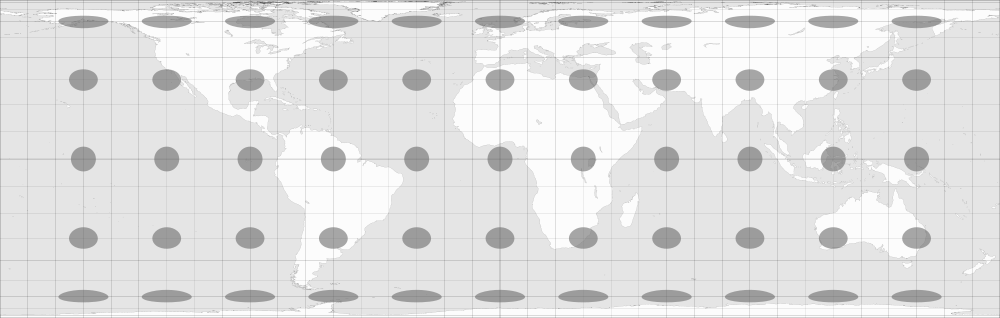
\includegraphics[width=0.9\linewidth]{graphics/basics/projection_distortion_lambert.png}
    \caption{equivalent Lambert projection \protect\footnotemark}
  \end{subfigure}
  \begin{subfigure}{0.39\textwidth}
    \centering
    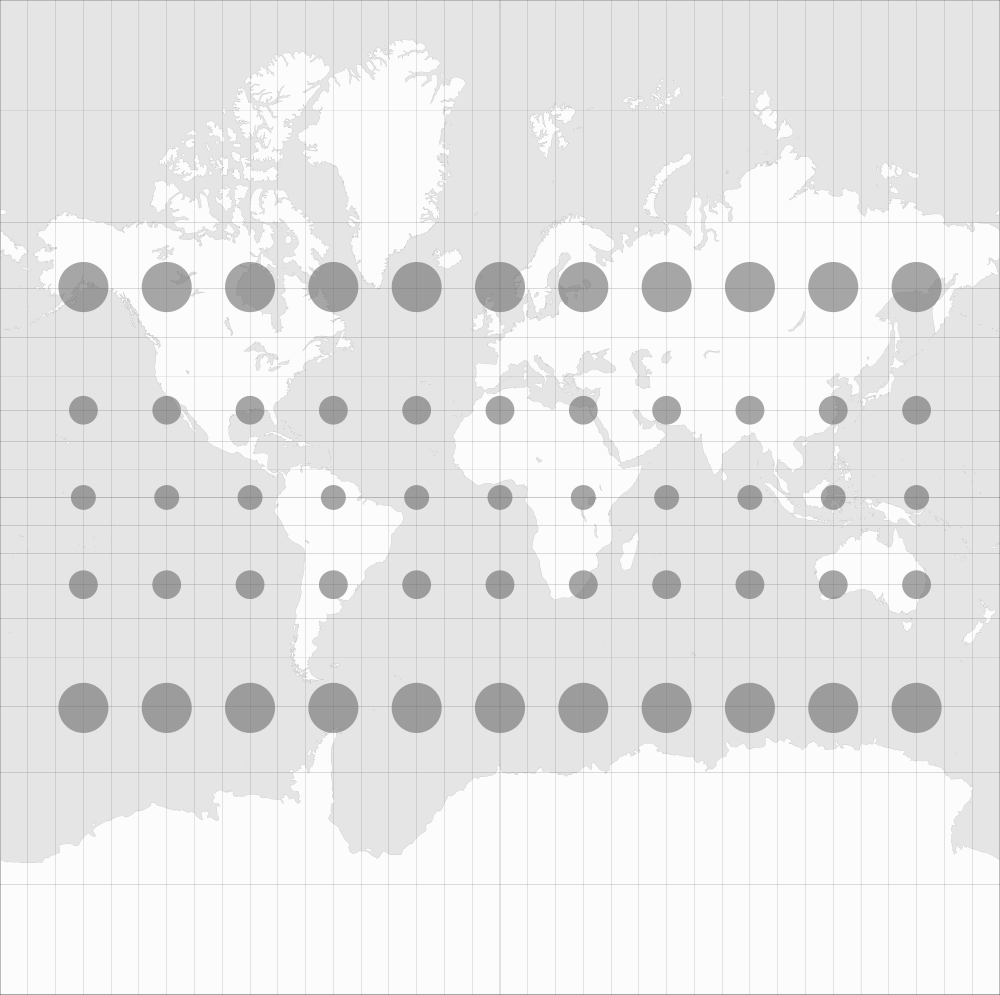
\includegraphics[width=0.9\linewidth]{graphics/basics/projection_distortion_mercator.png}
    \caption{conformal Mercator projection \protect\footnotemark}
  \end{subfigure}
  \caption{Comparison of equivalent and conformal map projections}
  \label{fig:lambert_vs_mercator}
\end{figure}

% reset footnotecounter by 1 (for left subfigure caption)
\addtocounter{footnote}{-1}
\footnotetext{
  \textit{Tissot indicatrix world map equirectangular proj},
  Eric Gaba / Sting (Wikimedia), June 2008
  URL: \url{https://commons.wikimedia.org/wiki/File:Tissot_indicatrix_world_map_equirectangular_proj.svg},
  last access: 28.10.2015
}

% set footnotecounter to next footnote (for right subfigure caption)
\addtocounter{footnote}{1} % count to next footnote
\footnotetext{
  \textit{Logo of the United Nations},
  Shizhao (Wikimedia), 13.06.2007
  URL: \url{https://commons.wikimedia.org/wiki/File:Logo_of_the_United_Nations_(B\%26W).svg},
  last access: 28.10.2015,
  Comment: This work is excerpted from an official document of the United Nations prior to 17. September 1987.
}

A compromise between preserving areas and shapes is the \emph{Robinson projection}. It is neither conformal, nor equivalent, but provides a reasonable trade-off between both properties.

\begin{figure}[ht]
  \centering
  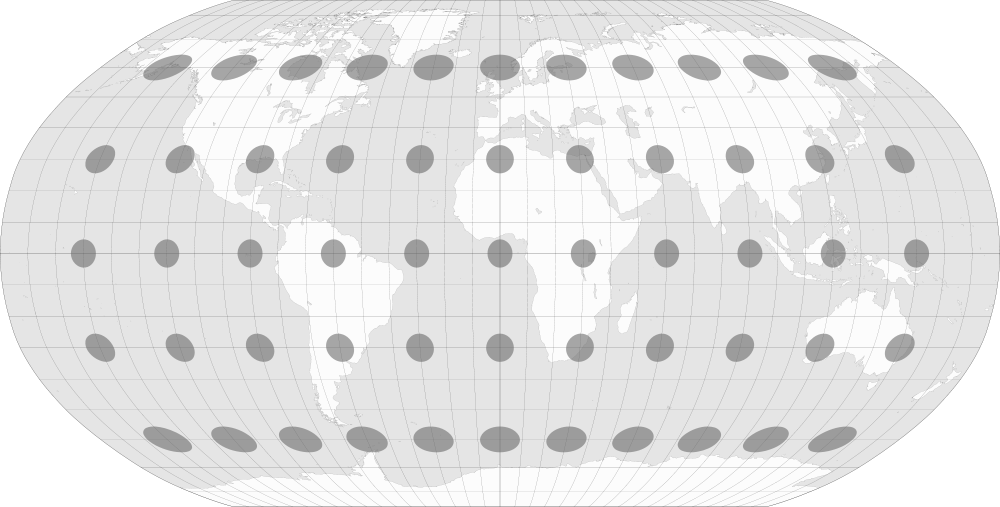
\includegraphics[width=0.65\textwidth]{graphics/basics/projection_distortion_robinson.png}
  \caption{Robinson projection \protect\footnotemark}
  \label{fig:robinson_projection}
\end{figure}

\footnotetext{
  \textit{Tissot indicatrix world map Robinson},
  Eric Gaba / Sting (Wikimedia), June 2008
  URL: \url{https://commons.wikimedia.org/wiki/File:Tissot_indicatrix_world_map_Robinson_proj.svg},
  last access: 28.10.2015
}

% paragraph map_projections (end)


% subsection presentation_of_geographic_space (end)


% ------------------------------------------------------------------------------
\subsection{Model of Historical Time} % (fold)
\label{sub:model_of_historical_time}

Time is an abstract concept that ``can be perceived only by its effects''
\cite[p. 27]{Langran1989timeingis}.
Many philosophers and scientists have been developing models to work with time. In this case, the model needs to be appropriate to both represent time in an historical sense in interplay with geographical space.

A popular model is \emph{Cartographic Time}, where time is seen as the ``fourth cartographic dimension'', is suitable for spatio-temporal information systems
\cite[p. 28]{Langran1989timeingis}.
Whereas space is represented by geo-objects on a map, time may be seen as versions or states on a timeline, separated by events that change one state to another state.
Unlike space, time knows only one dimension.
The position of an event on the timeline is described by its date using a reasonable sampling unit like century, year, day, hour or millisecond
\cite[p. 32]{Langran1989timeingis}.

% - - - - - - - - - - - - - - - - - - - - - - - - - - - - - - - - - - - - - - -
\paragraph{Types of Time} % (fold)
\label{par:types_of_time}

The simplest categorization is between a discrete \emph{event} and a continuous \emph{process}. Events can happen at a certain \emph{time point} or like processes in a \emph{time interval} or \emph{time period}, defined by two time points. An information system that stores events with a significant outcome regarding the geo-objects in the system, is an \emph{event-based historical geographic information system}. On the other hand, a \emph{process-based historical geographic information system} models mainly processes as a series of events of one kind regarding a small set of geo-objects
\cite[chapter 2, pp. 47-49]{solana2014spatio}.

The Taxonomic Model of Time by
\cite{frank98typesoftime}
classifies time not only into discrete and continuous, but also by the \emph{nature of time} or \emph{time order}: a consecutive development on the time axis, defined by start and end, defines \emph{linear time}. In a contrary, \emph{cyclic time} has no predefined order and events reoccur on a regular cyclic basis. The other two types, \emph{branching time} and \emph{multi-dimensional time}, are more complex and not relevant for this thesis.

% paragraph types_of_time (end)

% - - - - - - - - - - - - - - - - - - - - - - - - - - - - - - - - - - - - - - -
\paragraph{Temporal Topological Relations} % (fold)
\label{par:temporal_relations}

The topological relationship between two time points $t_1$ and $t_2$ is straightforward. Since they are discrete elements and therefore isomorphic to the number space of integers, there are three different order relations:
\begin{compactenum}
  \item $t_1 < t_2$: the first event happens before the second event
  \item $t_1 > t_2$: the first event happens after the second event
  \item $t_1 = t_2$: the first and the second event happen at the same time
\end{compactenum}

For time spans, there are six possibile temporal topological relations (table \ref{tab:temporal_relations}). Except for \texttt{equals}, each of them has an inverse, yielding a total of 13 different relations.

\begin{table}[H]
\begin{center}
\begin{tabular}{c c c}
    % \toprule
    relation & symbol & visualization \\
    \midrule
    $X$ before $Y$ &    \texttt{X < Y} & \raisebox{-0.25\height}
    {
\includegraphics{graphics/basics/temporal_relations/before}} \\
    $X$ meets $Y$ &     \texttt{X m Y} & \raisebox{-0.25\height}
    {
\includegraphics{graphics/basics/temporal_relations/meets}} \\
    $X$ overlaps $Y$ &  \texttt{X o Y} & \raisebox{-0.25\height}
    {
\includegraphics{graphics/basics/temporal_relations/overlaps}} \\
    $X$ equals $Y$ &    \texttt{X = Y} & \raisebox{-0.25\height}
    {
\includegraphics{graphics/basics/temporal_relations/equals}} \\
    $X$ starts $Y$ &    \texttt{X s Y} & \raisebox{-0.25\height}
    {
\includegraphics{graphics/basics/temporal_relations/starts}} \\
    $X$ during $Y$ &    \texttt{X d Y} & \raisebox{-0.25\height}
    {
\includegraphics{graphics/basics/temporal_relations/during}} \\
    $X$ ends $Y$ &      \texttt{X e Y} & \raisebox{-0.25\height}
    {
\includegraphics{graphics/basics/temporal_relations/ends}} \\
    % \bottomrule
\end{tabular}
\caption{Temporal relations of time spans, based on \cite{allen84}}
\label{tab:temporal_relations}
\end{center}
\end{table}

% paragraph temporal_relations (end)

% subsection model_of_historical_time (end)

% ------------------------------------------------------------------------------
\subsection{Presentation of Historical Time} % (fold)
\label{sub:presentation_of_historical_time}

In contrast to space, time does not have an intrinsic representation. However, the most common form to visualize cyclic time is on a cyclic display, e.g. a time wheel or a clock. Linear time is very often visualized on a \emph{timeline}. The purpose of a timeline is to show events as time points or processes as time intervals in chonological order. A timeline additionally shows time markers showing a certain date to support orientation. A timeline uses a certain time scale:

\begin{itemize}
  \item On a \emph{linear} timeline, the distance between any two time points is directly proportional to their actual temporal distance.
  \item A \emph{logarithmic} timeline uses a logarithmic function to scale the depicted time. Relative to a reference point on the timeline, e.g. the timeline center, the further away a time point, the further away its position on the timeline -- however, the distance between the time point and the reference point does not increasy linearily, but logarithmically. That means, events that are further away do not appear as far. This time scale accounts for logarithmic human perception: events that happened 20 years ago do not seem to be twice as long ago as events happening 10 years ago
  \cite{logorlinear}.
  \item A timeline can also have an \emph{irregular} scale, e.g. to have the same absolute distance of events on the timeline. This is useful if the distribution of the events on the timeline are far from homogeneous.
\end{itemize}

\begin{figure}[ht]
  \centering
  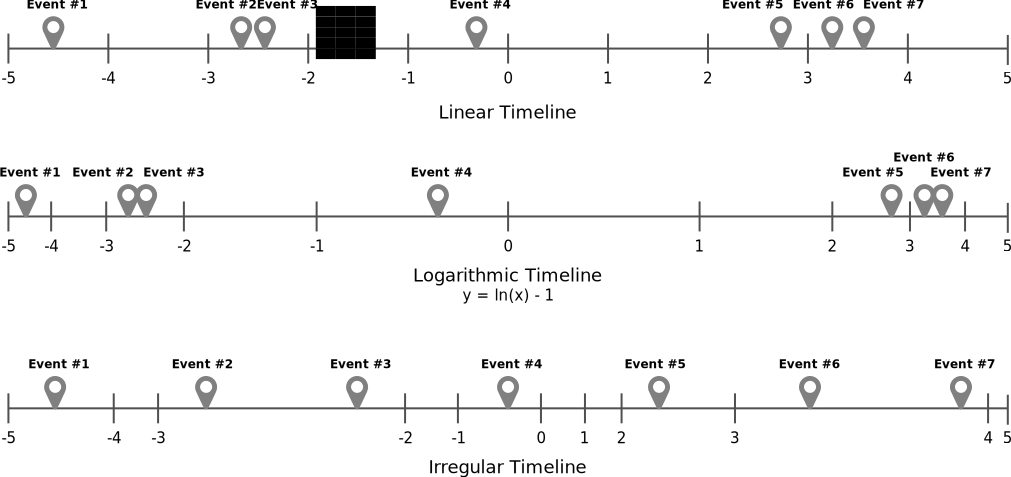
\includegraphics[width=0.8\textwidth]{graphics/basics/timelines/timelines}
  \caption{Comparison between a linear, a logarithmic and an irregular timeline}
  \label{fig:timelines}
\end{figure}

The visualization of time can be separate from the spatial dimension, according to the Triadic Framework, e.g. with a timeline. In another approach, space and time can also be coupled and displayed in the same presentation display, e.g. in a space-time cube \cite{haegerstrand1970}.


% temporal domain
%   linear time
%     time line
%     time series: graph (t,y coordinate system)
%     2.5D map: temporal dimension on z axis or on surface
%     space-time path
%   cyclic time
%     time series: polar diagram
%     time wheel
%   both
%     mono-temporal: one layer -> one time point
%     multi-temporal: one layer -> multiple time points
% \cite[p. 144]{ott2001time}

% subsection presentation_of_historical_time (end)

% section time_and_space (end)


% ==============================================================================
\section{Spatio-Temporal Data Models} % (fold)
\label{sec:spatio_temporal_data_models}
\begin{quoteit}
  ``Geography differs from geometry because \\
  in geography, space in indivisibly coupled with time''
\end{quoteit}
\hfill -- Don Parkes \& Nigel Thrift (1980)

A model tries to replicate a part of the real world. A data model abstracts a part of the world, identifies the most essential elements and their relation to each other. Historical Geographic Information Systems can be used to explain spatial-temporal phenomena in the real world. Therefore, it needs to handle the development of geo-objects and their attributes over time. Developments are driven by \emph{changes} to the state of an object.

Based on the theory of the \emph{Triadic Framework}, there are three components involved: space (3 dimensions), time (1 dimension) and attribute (multiple dimensions). All of these dimensions can change independently from each other
\cite[p. 53]{ott2001time}.
However, in order to trace spatial and attribute changes over time, the dimensions have to be related to each other.

% TODO: absolute time vs. relative time
% TODO: absolute space vs. relative space

Throughout the lifetime of a geo-object, it appears at some point, might undergo several changes and might disappear at some other time point. The data model has to be able to effectively and efficiently manage those changes. There are mainly two kinds: \emph{Discrete changes} are based on the idea of a \emph{state machine}: At any point in the lifetime, an object is in a certain state. It stays there until an event occurs that suddenly changes the object into a new state at a discrete time point. As an example, if an armistice agreement between two former war parties $A$ and $B$ contains a deal to cede parts of the territory of A to become territory of B, this territorial change is sudden. On a contrary, an object can gradually change according to a \emph{continuous process}, e.g. the change of the coastlines of landmasses
\cite{peuquet99}.

The spatio-temporal data models developed in the previous 30 years differ mostly in the organizing dimension: In \emph{location-based} models time is an attribute of a geo-object. On a contrary, \emph{time-based} approaches handle events and processes that change objects suddenly or gradually. \emph{Entity-based} models represent geo-objects as own entities. Spatial changes over time are related to these entities, but they are not attributes and therefore independent.


% The basis for all models is the concept of \emph{Time Geography} by
% \cite{haegerstrand1970}:
% Hägerstrand argued for an orthogonal relationship between time and space and that each object can be at one location only at one time. He furthermore visualized an objects development in a \emph{space-time path}. This section will introduce the most important \emph{spatio-temporal data models} (STDM) based on this idea that are releveant for the remaining parts of the thesis.
% TODO: version management (Wachowitz p 43)

This section introduces different spatio-temporal data models to maintain relations between time and space of an entity.

% ------------------------------------------------------------------------------
\subsection{Snapshot Model} % (fold)
\label{sub:snapshot_model}

One of the simplest, oldest and most frequently used models is based on the idea of \emph{snapshots}: At a certain time point $t_i$, a new layer gets created. It stores the full picture of the current state of all geo-objects
\cite{Langran1988frameworktgis}.

\begin{figure}[H]
  \centering
  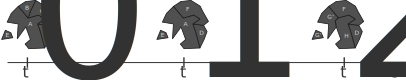
\includegraphics[width=0.8\textwidth]{graphics/basics/stdm/snapshot_model}
  \caption{The Snapshot Model by \cite{Langran1988frameworktgis}}
  \label{fig:snapshot_model}
\end{figure}

The model allows to retrieve the state of the system at a defined time point $t_i$. However, for all other time points $t \neq t_i$ that are not covered by a snapshot, it is impossible to retrieve the state of the system, because the data model does not record any changes. This is an integral problem of the model and can not be solved. The original model is also redundant, because objects that have not changed from one snapshot to the next one are duplicated. However, there have been improvements made, e.g. by \cite{armenakis92}.
Historical maps are examples for snapshots: They show the state of the world at one point in history, e.g. Europe 1919 and Europe 1945. However, with no additional information, it is impossible to deduct how Europe looked like in 1939. Therefore, this model is not suitable for the domain of this thesis.

% subsection snapshot_model (end)

% ------------------------------------------------------------------------------
\subsection{Simple Time-Stamping} % (fold)
\label{sub:simple_time_stamping}

This problem is solved by assigning a geo-object a period of existance by two additional attributes: at the \emph{start date} $t_{start}$ the object gets created and at the \emph{end date} $t_{end}$ it is ceased. If an object still exists its cessation date gets a special value, e.g. \texttt{NOW}
\cite{hunter90timestamping}.

\begin{figure}[ht]
  \centering
  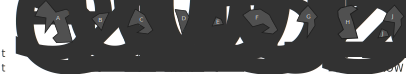
\includegraphics[width=0.8\textwidth]{graphics/basics/stdm/simple_time_stamping}
  \caption{The Simple Time-Stamping method by \cite{hunter90timestamping}}
  \label{fig:simple_time_stamping}
\end{figure}

The \emph{Simple Time-Stamping} method is also location-based and tracks discrete changes of objects. Given full and integer information, the state of the system at each time point $t_i$ can be retrieved: All geo-objects for which ~$t_{start} \leq t_i < t_{end}$~ are active, all others are inactive. However, this retrieval is cumbersome, because without efficient data structures every time the date changes, it has to be checked for each geo-object if its state has changed.

Another problem of the model is that it does not allow for tracing the development of objects in different states. As an example, at time point $t_1$ the geo-objects $B$ and $C$ cease and $G$ starts. Visually, $G$ is a successor of $B$ and $C$, but this historical relationship can not be deducted directly from the model. This shortcoming can be resolved by adding a reference to the predecessor and the successor of the object.

This model alone is not suitable for the domain of this thesis, because it is impossible to say what exactly has happened at a certain time point. Given the example above, it is unclear if two objects unified to a new one ($B+C \to G$) or if two are successors ($B \to G$) and one just stops to exist ($C \to \emptyset$). The model is also redundant: if a geo-object replaces another one ($B \to G$), then the end date of $B$ is the same as the start date of $G$.
% \cite[p. 46-47]{solana2014spatio}.

% subsection simple_time_stamping (end)

% ------------------------------------------------------------------------------
\subsection{Event-Based Spatio-Temporal Data Model} % (fold)
\label{sub:event_based_spatio_temporal_data_model}

A time-based approach addresses exactly those shortcomings: They explicitly represent events or processes in the data model and associate all objects that change according to them. One example of this approach is the \emph{Event-Based Spatio-Temporal Data Model} (ESTDM) for geospatial raster data by
\cite{peuquet95}.

At one defined time point $t_b$, a snapshot gets stored. This \emph{base map} contains the current state of the map, i.e. the current value of each raster cell \texttt{(x,y)}. From that moment on, the system stores events that change the values of certain cells. Such an event has a time stamp (\texttt{t}) and a list of components associated with it. A component represents a new value (\texttt{v}) and knows which raster cells (\texttt{x}, \texttt{y}) change their value to \texttt{v}.

The method uses the following data structures: a header file contains information about the thematic domain, a pointer to the base map and to the first and last element of the event list. This doubly-linked list stores all events chronologically. Therefore, each event knows its preceding and succeeding event via a \texttt{prev} respectively \texttt{next} pointer.
% TODO: graphic

If the time point of an event is reached, all its components are executed, i.e. the relevant raster cells change their value. The system follows the \texttt{next} pointer to know which event is waiting to be executed next. Since a change is relative to the previous change, not to the base map, change tracking is efficient.

The concept of the ESTDM suits the problem domain really well: An historical event changes the geometry of certain objects suddenly. The model explicitly represents these discrete changes. However, it does not work for vector data. The authors have explicitly stated that ``the design of such a [vector-based] model is not seen as a straightforward task'', because of the problem ``how to maintain the integrity of spatial topology as it changes [...] The solution will require a more complex definition of components within individual events''
\cite[p. 21]{peuquet95}.

% Also, just like the Simple Time-Stamping method, this model is only suitable for discrete but not for gradual changes. This problem is solved in the \emph{ObjectOriented geomorph} model by \cite{raperlivingstone95}.

% subsection event_based_spatio_temporal_data_model (end)

% ------------------------------------------------------------------------------
\subsection{Three-Domain Model} % (fold)
\label{sub:three_domain_model}

An event-based STDM for vector geometry including lines and polygons has to answer the following questions: What uniquely identifies a geo-object? What kind of spatial, topological and attribute changes can happen to an object? Which of these maintain the identity and which create a new object? This problem is addressed in the \emph{Three-Domain Model} by \cite{yuan96threedomain, yuan96temporal}. The model is based on abstract entities that represent a spatio-temporal object. It handles the three domains identity, space and time separately:
\begin{itemize}
  \item The \emph{semantic domain} holds an entity uniquely identifiable. An object in this domain corresponds to a human concept, e.g. a ``country''.
  % It handles attributes of the area, but not the spatial and temporal properties.
  \item The \emph{spatial domain} represents geospatial objects in vector format, e.g. a polygon describing the territory of a country.
  \item The \emph{temporal domain} stores all temporal objects, e.g. time points of an historical events, or time intervals of a war.
\end{itemize}

The model is not specific, but more a general abstract framework to handle space, time and identity. This makes the model very flexible, e.g. it can handle discrete and continuous changes, relative and absolute time, world and database time. One limitation of the model is that it only traces spatial attributes over time. In an alternative model by \cite{claramunt95timeingis}, the \emph{thematic domain} is added to fully describe a spatio-temporal object and trace also aspatial attributes that can change over time, e.g. the name of an entity.



Since countries, their territories and attributes can change independently over time, the data model used in this thesis will be built on top of the Three Domain Model.

% subsection three_domain_model (end)

% ------------------------------------------------------------------------------
\subsection{History Graph Model} % (fold)
\label{sub:history_graph_model}

Most of the data models introduced so far cover only static changes of geo-objects. \cite{renolen96} identified three different types of temporal behaviour of changing objects:
\begin{compactitem}
  \item Dynamic objects that change continuously.
  \item Static objects that change according to events with duration (processes).
  \item Static objects that change according to sudden events.
\end{compactitem}

Based on this observation he developed a data model that can handle all three kinds of temporal behaviour: The \emph{History Graph Model}. It manages objects and events separetly from each other. An object can only be in three different states:
\begin{enumerate}
  \item An object is \emph{static}, if it currently does not change. This is called an \emph{object version}. The version has an interval associated to it representing the duration of the object version, until it changes the next time. If the object is dynamic and changes continuously, the duration is zero.
  \item If an object is currently \emph{changing}, it is in an \emph{object transition}. The transition has an associated interval as well, whose duration is zero if it is a sudden change. Additionally, a transition links the relevant objects to each other creating a historical predecessor-successor-relationship.
  \item An object that is currently not active, is \emph{ceased} and not visible on the map.
\end{enumerate}

The history of a geo-object is a chronologically ordered set of versions and transitions, that can be visualized in a graph (see figure \ref{fig:history_graph_model}).

\begin{figure}[H]
  \centering
  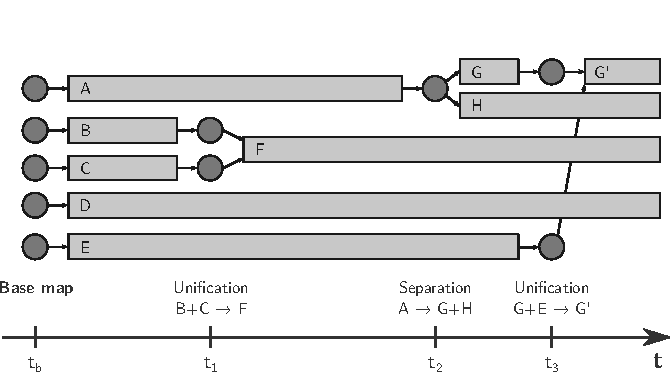
\includegraphics[width=0.8\textwidth]{graphics/basics/stdm/history_graph_model}
  \caption{The History Graph model}
  \label{fig:history_graph_model}
\end{figure}

The model defines six basic types of temporal changes that can happen (see figure \ref{fig:history_graph_changes}):
\begin{compactitem}
  \item \textbf{Creation}:           A new object is created.
  \item \textbf{Alteration}:         A property of an object (e.g. geometry) changes.
  \item \textbf{Cessation}:          An object is ceased.
  \item \textbf{Reincarnation}:      An object that has previously been ceased is recreated.
  \item \textbf{Split/Deduction}:    An object is divided into two or more new objects or one or more objects are deducted from an existing one.
  \item \textbf{Merge/Annexation}:   Two or more objects are joined together to a new object or one or more objects are annexed to another object.
\end{compactitem}

\begin{figure}[ht]
  \centering
  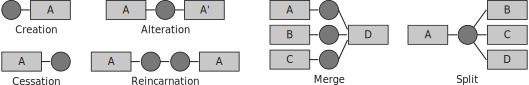
\includegraphics[width=0.8\textwidth]{graphics/basics/stdm/history_graph_changes}
  \caption{Types of changes in the History Graph model}
  \label{fig:history_graph_changes}
\end{figure}

The History Graph model can be seen as an extension to the ESTDM. It combines the advantages of event-based and entity-based spatio-temporal data models, supports discrete and continuous changes and relative and absolute time. The main improvement is that the historical development of a geo-object can directly be derived from the model, because objects are linked to their precedessors and successors --- the History Graph Model can tell a story. This is the reason why this model is particularly suitable for the work of this thesis.

% subsection history_graph_model (end)

\vspace{1em}
Other popular spatio-temporal data models that are not covered in this work, because they were not seen as relevant for the domain, include the \emph{Space-Time Composite} model, the \emph{Grid Model} and the \emph{Amendment Vector Model}. Overviews about these and other spatio-temporal data models can be found in \cite{zhao11}, \cite{pelekis04stdms} and \cite{peuquet99}.

% section spatio_tempora_data_models (end)


% ==============================================================================
\section{Database Management Systems} % (fold)
\label{sec:database_management_systems}

Information systems use databases for managing the data. A \emph{Database Management System} (DBMS) is a software system for the administration of data, mainly storage and retrieval. There are mainly two types of DBMS: the oldest and most common ones are \emph{Relational DBMS}. \emph{Object-Oriented DBMS} werde developed to adapt concepts of object-oriented programming into the database world. The combination of both approaches are \emph{Object-Relational DBMS}.

% ------------------------------------------------------------------------------
\subsection{Relational Database Management Systems} % (fold)
\label{sub:relational_database_management_systems}

RDBMS are built upon the concept of \emph{entitities}, e.g. an \texttt{HistoricalCountry}, with \emph{attributes}, e.g. \texttt{name} and attribute values of a simple data type, e.g. the character string \texttt{"Germany"}. Entities are represented in a table with one row for each \emph{tuple} and one column for each attribute. An entity has one attribute that unambiguously identifies each tuple, the \emph{primary key}, mostly a contiguous number.

Entities can be related to each other in three different kinds of \emph{relations}:
\begin{compactenum}
  \item[\texttt{1:1}] Direct attributional relation, e.g. one country has one head of state and vice versa.
  \item[\texttt{1:n}] One-to-many relation, e.g. one country can have many cities, but each city can belong to only one country.
  \item[\texttt{m:n}] Many-to-many relation, e.g. one country can have many rivers, but each river can also flow through multiple countries.
\end{compactenum}

Entities and their relations are visualized in an \emph{Entity-Relationship Model} (ER model). Data can be retrieved from and entered into a relational database using the \emph{Structural Query Language} (SQL). The query to get the names of cities in \texttt{Germany} in alphabetical order is:

\vspace{-1em}
\begin{verbatimtab}
  SELECT     city.id, city.name
  FROM       (city JOIN country ON city.country = country.id)
  WHERE      country.name = "Thüringen"
  ORDER BY   city.name
\end{verbatimtab}
\vspace{-1em}

The first RDBM developed was \emph{Oracle}, released in 1979 \cite{oracleDB}. Since then, the concept has been established as the state-of-the-art for databases. An example for a popular RDBMS used for Web-bases systems is \emph{MySQL}, the ``world's most popular open source database''
\footnote{
  \emph{MySQL :: About MySQL},
  URL: \url{https://www.mysql.com/about/},
  last access: 31.10.2015
}.


% subsection relational_database_management_systems (end)

% ------------------------------------------------------------------------------
\subsection{Object-Oriented Database Management Systems} % (fold)
\label{sub:object_oriented_database_management_systems}

One problem with RDBMS is that attributes can only be assigned simple data types. Developers using object-oriented programming need to map the objects used in the application to tuples in the relational database -- and vice versa data from the database needs to be transformed to objects in the application. This process can be cumbersome. OODBMS have been developed to address this problem and adopt the concepts of object-oriented programming for database management purposes \cite{oodbms}.

\begin{itemize}
  \item \emph{Classes} are the structured representation of things in the real world of the same kind, with the same properties, e.g. a country, having a name and a territory. Classes in OODBMS relate to Entities in RDBMS.
  \item An \emph{object} is an instance of a class, one specific thing with defined properties, e.g. the country of Germany with its territory. This correlates to a tuple in RDBMS.
  \begin{itemize}
    \item The \emph{attributes} of an object can not just be of a simple data type, but also instances of other classes, e.g. \texttt{country.territory} can be a \texttt{polypolygon} object. These complex data types are a major improvement compared to RDBMS.
    \item Objects also have \emph{methods} that can be called to do something with the object, e.g. \texttt{territory.getArea()} calculates the area size of a country.
  \end{itemize}
  \item The internal state of an object can not be accessed from the outside. Methods are the only way to interact with an object. This is called \emph{encapsulation} and maintains control over what can be done to and with an object and prevents corruption.
  \item According to the concept of \emph{inheritance}, classes can be hierarchically structured, whereas the attributes and the methods of a \emph{base class} are inherited to its \emph{derived class}. As an example, an \texttt{Area} has a \texttt{name}, a \texttt{territory} and the method \texttt{getArea()} associated to it. A \texttt{Country} can be derived from the \texttt{Area}, inheriting both attributes and the method. Additionally, it can get an attribute \texttt{head\_of\_state}, which is specific to \texttt{Country}, but not to \texttt{Area}. The class \texttt{Ocean} can just as well be derived from \texttt{Area}.
  \item An associated concept is \emph{polymorphism}: The same function can be called on different objects and the return value will be of the same type. However, internally it might be calculated differently. As an example, consider the classes \texttt{Polygon} and \texttt{Polypolygon}, both inherited the method \texttt{getArea()} from their base class \texttt{Geometry}. Whereas a polygon calculates its area directly based on its geometry, a polypolygon internally calles the function \texttt{getArea()} on all its associated polygons and sums up their areas.
\end{itemize}

OODBMS support all those concept and allow to store the objects used in the application directly in the database. Additionally, objects from the database can be accessed directly, there is no need for an additional query language \cite{oodbms}.

% subsection object_oriented_database_management_systems (end)

% ------------------------------------------------------------------------------
\subsection{Object-Relational Database Management Systems} % (fold)
\label{sub:object_relational_database_management_systems}

ORDBMS combine the advantages of both worlds. Internally, it uses the established and efficient relational database for the data storage. The database model and the interaction with the data happens in an object-oriented way while supporting all of the concepts mentioned in the previous subsection \ref{sub:object_oriented_database_management_systems}. The most popular ORDBMS example for Web-based systems is \emph{PostgreSQL}, ``the world's most advanced open source database''
\footnote{
  \emph{PostgreSQL:},
  The world's most advanced open source database,
  URL: \url{http://www.postgresql.org/},
  last access: 31.10.2015
}.

% subsection object_relational_database_management_systems (end)

% ------------------------------------------------------------------------------
\subsection{Spatio-Temporal Databases} % (fold)
\label{par:spatial_databases}

Databases for HGIS have to deal with spatial, temporal and attribute data. According to the Triadic Frame, these aspects should be modeled separately from each other, as they can change independently.

% - - - - - - - - - - - - - - - - - - - - - - - - - - - - - - - - - - - - - - -
\paragraph{Spatial data} % (fold)
\label{par:spatial_data}

can easily become very large, because of the mass of very precise coordinate data. \emph{Spatial databases} are specialized to work with spatial data: they process the data effieciently and to provide general data types, such as \texttt{Point} or \texttt{Polygon} and methods, e.g. to calculate the area or the distance between two points. \emph{PostGIS}
\footnote{
  \emph{PostGIS},
  URL: \url{http://postgis.net/},
  last access: 31.10.2015
}
is an extension for PostgreSQL that is especially utilized for handling spatial data.

% paragraph spatial_data (end)


% - - - - - - - - - - - - - - - - - - - - - - - - - - - - - - - - - - - - - - -
\paragraph{Temporal data} % (fold)
\label{par:temporal_data}

usually relates to events and processes. It is defined either by a time point or a time interval which is again defined by two time points. This is called a \emph{bitemporal} element. A time point can be modeled in the database as an attribute of the complex \texttt{Date} type. For relational databases that only support simple data types, the date can be stored as a string or be expressed with a \texttt{long} integer (64 bit) $\forall n \in \mathbb{N}: n \in [-2^{63}~..~2^{63}-1]$) determining the number of milliseconds since \nth{1} January 1970 (UNIX time) \cite{timeInRDBMS}. SQL was extended by features to handle time in a database, e.g. \emph{SQL/MM} \cite[chapter 6]{peuquet99}.

% paragraph temporal_data (end)

% - - - - - - - - - - - - - - - - - - - - - - - - - - - - - - - - - - - - - - -
\paragraph{Object-Oriented Spatio-Temporal Database Models} % (fold)
\label{par:object_oriented_spatio_temporal_database_models}

The question is: How to implement the spatio-temporal data modles introduced in section \ref{sec:spatio_temporal_data_models} in a relational, object-oriented or object-relational database management system introduced in this section? While the implementation depends on the data model, there are common concepts and isses that have to be addressed.

When storing time related data, it is important to distinguish between the time that was true in reality (\emph{valid time} or \emph{world time}) and the time it was stored in the database (\emph{transaction time} or \emph{database time}). A property of spatio-temporal database models is whether valid and transaction time are supported.

Object-oriented concepts are more appropriate than the concept of relational databases, because of the complex nature of spatio-temporal data \cite[section 3.9]{pelekis04stdms}. One of the first concepts was the concept of a \emph{spatio-temporal object} combining geometrical and bitemporal properties in one object \cite{worboys90stdm}.

A similar approach by \cite{raza12} is the \emph{Spatio-Temporal Data Type} (STT). Time is not considered an attribute of space, but a separate class. They are aggregated in the \texttt{SpatioTemporal} class, using both spatial and bitemporal attributes. The model also provides spatio-temporal operators, e.g. \texttt{STT\_intersects} returns \texttt{true} if two \texttt{SpatioTemporal} objects intersect in time and space, i.e. their geometries intersect and the time intervals in which they are active overlap. These operators are very helpful when analyzing spatio-temporal data or checking for data integrity.

% paragraph object_oriented_spatio_temporal_database_models (end)

% - - - - - - - - - - - - - - - - - - - - - - - - - - - - - - - - - - - - - - -
\paragraph{Version management} % (fold)
\label{par:version_management}

An issue is how to perform retrospective updates. Given a database model that stores objects that are created, updated and destroyed by events. Object $X$ is created at time point $t_x$. At time point $t_y$, $X$ gets destroyed and replaced by object $Y$. If a new change that updates $X$ to $X'$ gets inserted at time point $t_u$ in between, i.e. $t_x < t_u < t_y$, then the event at time point $t_y$ is not correct anymore, because object $X$ does not exist. The question is how to maintain data integrity on insertion, update and deletion from a spatio-temporal database? This issue has to be addressed using formal logic for temporal reasoning
\cite[section 6]{peuquet99}.

% One approach to handle this issue is \emph{version management}, introduced by
% \cite WH94
% There are \emph{object version} and \emph{object configuration}. The concept is based on four premises:
% \begin{compactenum}
%   \item Each object must have an initial version.
%   \item The versions of an object are hierachically structured.
%   \item One object version relates to exactly one object instance and vice versa.
%   \item There is always one current version of an object.
% \end{compactenum}

% Throughout time, a set of interrelating object versions is created. They are handled by four update procedures that create new object versions:
% \begin{compactenum}
%   \item Create of a new object.
%   \item Clone an existing object.
%   \item Update spatial attributes of an existing object (geometric change).
%   \item Update aspatial attributes of an existing object (thematic change).
% \end{compactenum}

% paragraph version_management (end)


% \cite[p. 69]{ott2001time}.

% section database_management_systems (end)

% ==============================================================================
\section{HistoGlobe} % (fold)
\label{sec:histoglobe}


Application: HistoGlobe
A distributed \emph{Web Information System}, consists of a remote server side, on which the storage and management of the actual data happens, and the client side on which the user communicates with the system. It hosts the user interface that is rendered in a Web browser.

map for spatial domain (x, y)
timeline for temporal domain (t)
-> 3D system

describe the components of the HG explicitally

ancestors successors
layers of administrative units
open to extension for additional attribute data (e.g. statistics)

requirements
  geographical knowledge
  contextualize / intersect historical sources
  accept imprecision
  prevent illusion of certainty

usable User Interface for both navigation and editing
-> problem: all interfaces are trés horrible!

module system


% section histoglobe (end)

% chapter bascis (end)

% ==============================================================================
\vspace{2em}

transition to concept chapter
